%Chapter 4

\renewcommand{\thechapter}{4}

\chapter[Improving the Posterior Estimates]{Estimating the posterior with an improved 
version of bootstrap sampling based on Equivalence Classes} 
\label{chapt4}

\section{Overview}
% talk about bayesian bootstraps
Rubin~\citep{rubin1981bayesian} introduced the Bayesian Bootstrap procedure, which generalizes 
the bootstrap and introduces a procedure for placing a prior over the sampling weights used in 
bootstrap resampling. The classic bootstrap is the posterior mean of the Bayesian bootstrap, and 
Rubin demonstrated they have quite similar estimation properties, generality, and similar 
limitations.

In particular, in the discussion of the paper introducing the Bayesian Bootstrap, when 
discussing model specification, Rubin muses:

\textit{``is it reasonable to use a model specification that effectively assumes all possible distinct 
values of X have been observed?"}

Specifically, both the non-parametric bootstrap and the Bayesian Bootstrap make this assumption — 
no unobserved value will ever be included in a bootstrap replicate. This renders unobserved 
values ``impossible'' under the model, and prevents understanding the effect they might have on 
the inference procedure or the estimator being computed.

% talk about how we wanna estimate the bayesian bootstraps
Here, we introduce the notion of the Augmented Bootstrap. This procedure follows the general 
framework of the bootstrap (or, optionally, the Bayesian Bootstrap), but augments the observed 
data with additional ``pseudo-observations'' that represent values that are possible given a 
conceptual model for data generation, but which were not observed in the sample.

\section{Methods}

We will explain this idea in the underlying context of the problem of quantifying the abundance 
of transcripts from RNA-sequencing (RNA-seq) data.  In this problem, we observe a collection of 
sequenced fragments, from which we can then estimate the abundance of the distinct transcripts 
using an expectation-maximization procedure (our ``estimator'' in the case of the bootstrap).  
Consider that we observe a collection $\mathcal{F}$ of $N$ sequenced fragments. Each fragment aligns 
to a set of distinct locations which we denote as $a(f_i) = \{(j_1, k_1), (j_2, k_2), \dots\}$ 
signifying that fragment $f_i$ aligns to transcript $j_1$ at position $k_1$, to transcript $j_2$ 
at position $k_2$, and soforth.  For a given set $\mathbf{\eta}$ of transcript abundances, we can 
write the probability of observing the set $\mathcal{F}$ of fragments as:

$$
\mathcal{L} = \prod_{i=1}^{N} \sum_{(j,k) \in a(f_i)} P(t_j|\mathbf{\eta}) P(f_i|t_{j,k}=1)
$$

where $P(t_j|\mathbf{\eta})$ is the probability of selecting transcript $t_j$ for sequencing 
conditional on the transcript abundances and $P(f_i|t_{j,k}=1)$ is the probability of generating 
fragment $i$ from transcript $j$ at position $k$.

% \textcolor{red}{is there a way to put $k$ on the left side of the conditional bar? it seems funny on the 
% right side in the second term}

While there is no closed-form solution to determine the $\mathbf{\eta}$ that maximize $\mathcal{L}$, 
we can, at least locally, optimize this quantity using an EM algorithm.  We are then interested in 
assessing the accuracy of $\mathbf{\hat{\eta}}$, our maximum likelihood estimator for $\mathbf{\eta}$.

To assess this accuracy, we can use the non-parametric bootstrap. In this framework, we will 
resample (with replacement) from $\mathcal{F}$ to produce a series of bootstrap replicates 
$\{\mathcal{F_1}, \mathcal{F_2}, \dots \mathcal{F_b}\}$, and for each we can use the EM procedure 
to obtain a maximum likelihood estimate of the transcript abundances given this bootstrap replicate; 
we denote these esitimates as 
$\{\mathbf{\hat{\eta_1}}, \mathbf{\hat{\eta_2}}, \dots, \mathbf{\hat{\eta_b}}\}$. 
We can then assess e.g. the variance of the estimate for the abundance of transcript $j$, denoted as 
$\hat{\eta}^{(j)}$, by assessing the sample variance of 
$\{ \hat{\eta_1}^{(j)}, \hat{\eta_2}^{(j)}, \dots, \hat{\eta_b}^{(j)} \}$.

Because we are resampling \textit{sequenced fragments} with replacement, we will never observe in our 
resampling a pattern of alignments for a fragment different from what we saw in our original sample 
$\mathcal{F}$. This leads to some interesting, and perhaps undesirable behavior of the bootstrap. 

Consider a pair of alleles of a transcript that differ only at a single locus.  Further, imagine 
that these transcripts are sequence distinct from the rest of the transcriptome (i.e. they share no 
multimapping reads with other transcripts apart from their sibling allele).  Let there be $N_t$ 
reads that map to both of these transcripts, and $0$ reads that map uniquely to either (i.e. 0 
reads that overlap the variant locus).

From the perspective of our estimator, these transcripts are inferentially indistinguishable.  
Specifically, with no prior information on whether one of these alleles is \textit{a priori} more likely 
than the other, we have no information about how the $N_t$ fragments should be allocated among 
these transcripts.  Perhaps $t_p$ and $t_m$ each give rise to $\frac{N_t}{2}$ fragments (what the 
EM will likely tell us), or perhaps $t_p$ gives rise to 0 fragments and $t_m$ gives rise to all 
$N_t$ fragments.  In fact, any combination between the two alleles that sums to $N_t$ is feasible 
and has equal likelihood.

The crux of the issue in uncovering this uncertainty using the non-parametric bootstrap (either the 
traditional or the Bayesian variant) is that no observation was made that distinguishes between 
these alleles.  Thus, no matter how we resample the original observations, we will never be able 
to recover the underlying uncertainty in the abundance of these transcripts.  Our estimator will 
demonstrate some variance over the bootstrap replicates, of course, but only related to what 
fraction of the original $N_t$ reads we sample within each replicate (with the expected value, 
of course, being $N_t$).

\subsection{The Augmented Bootstrap}

To address this issue, we propose the augmented bootstrap.  This procedure is applicable in 
situations where the data over which inference is being performed have a finite (and ideally ``small'') 
support. % **Mike: I think of the parameter having support, not data**  
We describe the procedure in 
full generality, and then explain the heuristics that we adopt to make the procedure computationally 
expedient in our use case.

The main idea behind the augmented bootstrap is that we will augment our observed data with some set 
of ``pseudo-observations'' --- data values that \textit{might} have been observed, but which were not observed 
in our sample.  This is analogous to placing a prior over the discrete set of possible observations 
that may be made. The prior may be informative or noninformative, and this can be represented by means 
of the sampling weights assigned to each of these pseudo-observations.

Let us consider our chosen problem of transcript abundance from RNA sequencing data. To simplify the 
exposition, let us further assume we are dealing with single-end reads, and that we will ignore the 
possibility of sequencing error when generating our ``pseudo-observations''. Then, in this case we 
may consider producing a set of pseudo-observations by drawing, from every transcript, a fragment 
starting at every position.  Let this set of pseudo-observations be denoted as $\mathcal{P}$ and 
let us denote by $\mathcal{F_{A}}$ the set $\mathcal{F} \cup \mathcal{P}$. This is our collection 
of augmented observations — the set of samples over which we will perform our augmented 
bootstrapping procedure.  While we could consider every observation $f \in \mathcal{F_{A}}$ to be 
sampled with replacement with equal probability, this introduces an obvious dependency between 
$\left|\mathcal{F}\right|$ and $\left|\mathcal{P}\right|$ where the effect of the 
pseudo-observations will be relatively larger when the original sample is small and less important 
when the original sample is very large.  Thus, we will consider modifying the sampling weights 
between ``true'' observations (those in $\mathcal{F}$ ) and pseudo-observations 
(those in $\mathcal{P}$).  While we can consider giving each pseudo-observation a distinct sampling 
weight, let us consider here the simpler case where we define $w < 1$ to be the sampling weight 
applied to every pseudo-observation.  In fact, this gives us a direct way to interpret the weight 
of all pseudo-observations as a proportion of the weight of the true observations.  Consider that 
we want the pseudo-observations to account for $1\%$ of the samples in a given bootstrap sample — 
then we can set the weights in the following way.

Let $\left|\mathcal{F}\right| = N$ and $\left| \mathcal{P} \right| = N'$ so taht 
$\left| \mathcal{F_{A}} \right| = N + N'$.  We would like the weight of each pseudo-observation 
to be proportional to $w$ times the weight of each true datum, where $0 \le w \le 1$. 
% Then we can say $\gamma = \frac{N}{N+N'} + \frac{w N'}{N+N'}$.

Now, when we perform a bootstrap replicate, we wish to resample with replacement from 
$\mathcal{F_{A}} = \langle f_1, f_2, \dots, f_N, p_1, p_2, \dots, p_{N'} \rangle$ where we will use 
the sampling weights $\langle y_1, y_2, \dots, y_N, z_1, z_2, \dots, z_{N'}\rangle$ where 

$$
% y_i = \frac{\gamma^{-1}}{N+N'}
y_i = \frac{(1-w) (N+N')}{N}
$$

% and 

$$
% z_i = \frac{w \gamma^{-1}}{N+N'}
z_i = \frac{w (N+N')}{N'}
$$

% This gives every pseudo-observation a relative sampling weight equal to $w$ times the sampling weight 
% of a true observation. 
This gives the relative sampling weight of every pseudo-observation and every true observation
equal to $w$ and $1-w$ respectively. Thus, in expectation, $(100 \times w)\%$ of our sampled data 
in each bootstrap replicate will consist of pseudo-observations, while the rest will consist of 
true observations.

The effect of adding these pseudo-observations to augment our bootstrap sampling is that we can now 
observe outcomes in our estimates that previously would have not been possible due to plausible 
observations that were missing from our specific sample.

Returning to the running example of the alleles of a single transcript; in addition to the $N_t$ 
fragments compatible with both alleles, there will now be pseudo-observations compatible only with 
$t_m$ and pseudo-observations compatible only with $t_p$.  In a given bootstrap replicate the 
inclusion or exclusion of these pseudo-observations will result in a different relative estimate 
between the abundances of these two alleles than we will ever arrive at under a bootstrap replicate 
of the original data.  In a sense, this augmentation is enabling us to approach the bootstrap 
procedure from a more Bayesian perspective, where data are \textit{possible} even when they are not 
observed.  The cost for this, of course, is that we must make some decision about their prior probability.

\subsection{Heuristics for augmenting the bootstrap}

We have defined the augmented bootstrap procedure as augmenting the observed sample with 
pseudo-observations for \textit{all possible} observations. This can immediately pose some challenges. 
First, it requires that the set of possible observations is finite and sufficiently small to be 
enumerated. Second, many possible pseudo-observations, though technically possible given the 
imposed prior, may have little to no effect on the resulting inference of interest.

Again, consider our running example of transcript abundance estimation. Here, under observations 
of the original sample, many transcripts will both have an estimated abundance of 0 and, further, 
will simply have no observed sequenced fragments compatible with them.  Generating and possibly 
sampling pseudo-observations from these transcripts may lead to small fluctuations in the estimated 
abundance of these transcripts across bootstrap replicates, but it is unlikely to have any 
substantial effect on the "main" inference problem (i.e. the estimated maximum likelihood 
abundances of non-trivially expressed transcripts) — and since no "true" observations are 
compatible with these transcripts, we'd expect their posterior samples to be rather uninteresting.

This immediately suggests one potential heuristic for limiting the number of pseudo-observations 
with which we will augment our true samples. Let $\mathcal{T}$ be our complete set of transcripts 
and let $\mathcal{T}_\mathcal{F}$ be the set of transcripts having at least one fragment in 
$\mathcal{F}$ that aligns to them. Rather than generating pseudo-observations from all of 
$\mathcal{T}$, we may consider generating pseudo-observations only from 
$\mathcal{T}_\mathcal{F}$ — that is from transcripts that we predict to be expressed and from those 
that have compatible observations (but which we may not predict to be expressed in the maximum 
likelihood estimate). In general, this will produce far fewer pseudo-observations than if we 
generate them from all of $\mathcal{T}$. Furthermore, the sampling of \textit{these} 
pseudo-observations are much more likely to lead to alternative high-likelihood estimates across 
bootstrap-replicates, because they are most likely to change the balance of observations in 
highly-ambiguous components within the inference problem. Thus, we are, in effect, selecting a 
smaller set of pseudo-observations that are more likely to uncover the relevant uncertainty 
in our estimator.

%\textcolor{red}{talk about just sampling from the single-transcript equivalence classes — that is, 
%While 
%We can take this idea one step further by, instead of generating pseudo-observations only from 
%$\mathcal{T}_\mathcal{F}$, only generating those \textit{specific} pseudo-observations from along 
%the transcripts in $\mathcal{T}_\mathcal{F}$ that are unique to each transcript.



\section{Results}

We have created a simulated dataset of Drosophila with an expression of the reads from two alleles of 
each gene. To create the allelic reads, we flip a random base in the original genes and then generate
reads with \polyester RNA-seq simulator~\citep{frazee2015polyester} from both allelic genes. Based on the 
procedure for generating the allelic reads, most, if not all, the reads mapping to a transcript, map 
to both its paternal and maternal alleles. We demonstrate how the \aboot improves the accuracy of abundance
estimation on a sample with high levels of ambiguity.


\begin{figure}
    \centering
    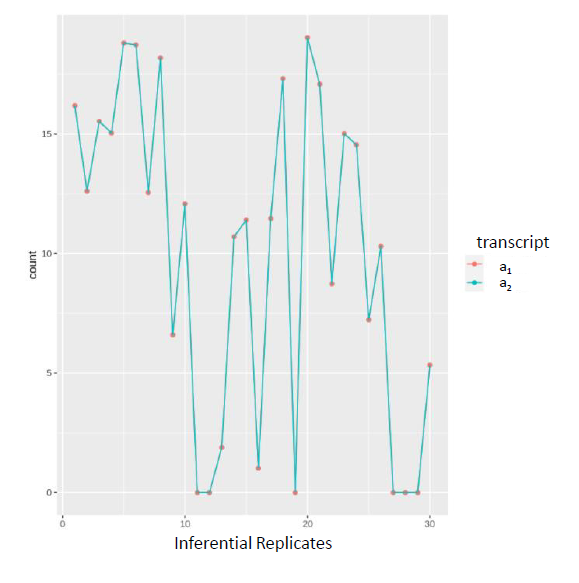
\includegraphics[width=0.4\textwidth]{{{Figures/aboost/w0}}}
    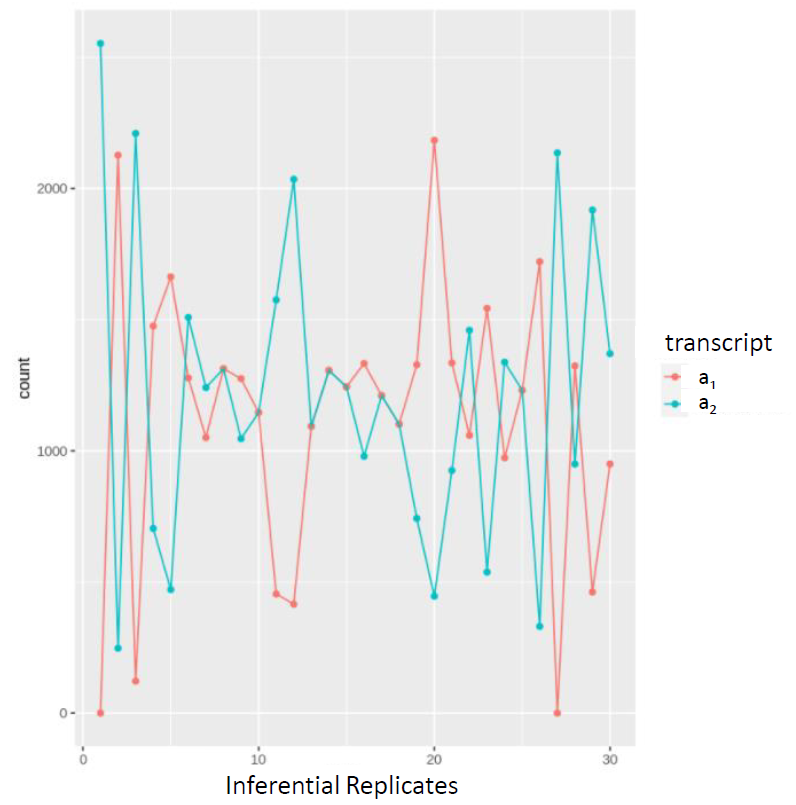
\includegraphics[width=0.4\textwidth]{{{Figures/aboost/w01}}}
    \caption[estimating uncertainty in two alleles of the same transcript]
    {The regular bootstraps do not capture any uncertainty in relative expression of two alleles
    of the same transcript. Using the augmented bootstrap improves uncertainty estimation.}
    \label{fig:al}
  \end{figure}
  

\subsection{Estimating the allelic expression of a simulated sample}

% TODO
% talk about the simulation process
To investigate how the posterior sampling could improve the accuracy of the abundance estimation, we follow 
a specific procedure for creating the multi-allelic RNA-seq sample from the Drosophila genome. %The simulation 
We assume the original genome is one parental allele, and generate the second allele by
adding a random mutation to 5 exons of each gene.

To increase the uncertainty in the abundance estimations, we simulate reads from both alleles of every
transcript in the reference transcriptome. Each transcript in the paternal allele is expressed by 
two reads. Then we select 1000 transcripts from each gene with 3 to 6 isoforms and alter the 
expression of the maternal allele of the transcript randomly in a way that the final gene count of the 
maternal allele will have the same expression level as the paternal allele.

We should acknowledge that the way this data is simulated is unrealistic because each transcript has
multiple alleles in the sample and all the transcripts are expressed. The reason, we follow the procedure
is to include a very high level of uncertainty so that estimating the posterior distribution becomes
more challenging.

First we simulated a small  sample and looked at the relative expression of two alleles of the
same transcript. We observed that the regular bootstrap estimate the expression of two alleles
to be the same in all the inferential replicates. This means that all the reads mapping to these alleles
are always separated equally to both sequences in all the bootstrap samples. This has been displayed
in~\cref{fig:al}. This figure also shows how using the augmented \boots with $w=0.01$ estimates the 
existing uncertainty for the relative expression of these two alleles properly. Because of the unique
reads that are sampled in some inferential replicates from each alleles, the multi-mapping reads
are not always equally distributed between the two alleles and their expressions are not always 
the same in all the inferential replicates.


Then we created a larger simulated sample with 30 M reads. In this sample,
we demonstrate how the regular \boots fail to capture the entire posterior distributions
for many \txps in this sample. We create inferential replicates by \boots available in \salmon and 
\kallisto. We also create \boot samples using the \aboots with different weights. We ran \salmon in two
different optimization modes of `EM' and `VBEM'. The `EM' mode is the regularly expected maximization 
algorithm and the `VBEM' is a variational bayesian version of the EM with non-zero priors for the 
model's parameters which induces further sparsity on the final solution.

\begin{table} \centering
    \begin{tabular}{lr}
    \toprule
    Method  & Spearman Correlation \\
    \midrule
    \kallisto & \num{0.9393075}  \\
    \kallisto \boot & \num{0.942153293871728}\\

    \salmon EM point-estimates & \num{0.9537012}  \\
    \salmon VBEM point-estimates & \num{0.7967372}   \\

    \salmon VBEM regular \boot  & \num{0.9010147} \\
    %\salmon VBEM \aboot (w=0.005) & \num{0.977737}  & \num{0.} \\
    \salmon VBEM \aboot (w=0.01) & \num{0.9852121} \\
    \salmon VBEM \aboot (w=0.1) & \num{0.9924701}  \\
    
    \salmon EM regular \boot  & \num{0.9561436}  \\
    %\salmon VBEM \aboot (w=0.005) & \num{0.}  & \num{0.} \\
    \salmon EM \aboot (w=0.01) & \num{0.986101}  \\
    \salmon EM \aboot (w=0.1) & \num{0.9924477} \\
    \bottomrule
    \end{tabular}
    \captionof{table}[Quantification of allelic transcriptome]{
        Accuracy of abundance estimation based on the Spearman correlation
        between the truth and the mean of the posterior distrubtion.
        Using the mean of the posterior distribution generated by
        \aboots with weight 0.01 and 0.1 significantly improves the 
        accuracy in the allelic expression quantification with RNA-seq.
    }
    \label{tab:allele}
\end{table}


\Cref{tab:allele} shows the performance of allelic expression quantification with both point estimates
and the mean of the posterior distributions. We observe that using the \aboots with both 0.01 and 0.1
weights increase the accuracy of the abundance estimation. This suggests that augmenting the sample with
one unique read for each possible transcript increases the ability of the uncertainty estimation with \boots.

We also evaluated the performance of the two optimization 
methods `EM' and `VBEM'. Because of the sparsity imposed by `VBEM' and the specific characteristics
of the simulated sample that almost all the transcripts are expressed, the point estimates calculated
by `VBEM' become less correlated with the truth. However, we observe that using the mean of the 
posterior distribution, both `EM' and `VBEM' reach a very high correlation with the truth.


To further investigate the effect of the \aboots for recovering the posterior distribution,
we evaluated the confidence intervals calculated based on both regular \boots and \aboots.
In this analysis, we look at confidence intervals with different lengths (0 to $100\%$) and at 
each level we calculate how many times the truth is found in that interval. 
%A good estimation of the posterior distribution should be able to recover the truth as many
If we have the true posterior distribution, the truth should be found in each interval 
relative to the length of the interval, e.g., if we are looking at the $95\%$ confidence interval,
we should be able to find the true value of the abundance at least $95\%$ of the time.

\Cref{tab:cnfint} shows the percentage of the transcripts at each level for which the truth
is recovered in the corresponding interval. We observe that either optimization method
using a pseudo-observation with $1\%$ reaches an empirical posterior distribution similar
to the theoretical distribution, specifically in the largest interval.
The highest similarity between the empirical and theoretical distribution 
is achieved at the $95\%$ confidence interval of the \aboots with $w=1\%$.
As we observed earlier, increasing the pseudo-observation weight to $10\%$ increased the spearman
correlation of the mean with the truth, however, in this evaluation we observe that sampling too
many reads from the pseudo-observation do not lead to an improved estimation of posterior distribution.


\begin{table} \centering
    \begin{tabular}{lrrrrr}
    \toprule
    Confidence interval length  & $5\%$ & $25\%$ & $50\%$ & $75\%$ & $95\%$ \\
    \midrule

    \salmon VBEM regular \boot  & \num{0.06384082 } & \num{0.2959801 } & \num{0.5404584} & \num{0.7455006 }& \num{0.888185 }\\
    \salmon VBEM \aboot (w=0.01) & \num{0.06804504 } & \num{0.3315576 } & \num{0.6126213 } & \num{0.8204567 }& \num{0.9416736}\\
    \salmon VBEM \aboot (w=0.1) & \num{0.02794655}  & \num{0.1451176} & \num{0.2990612} & \num{0.4785613}& \num{0.6842802}\\
    
    \salmon EM regular \boot  & \num{0.06063006 }  & \num{0.2872837} & \num{0.5227345 } & \num{0.7248395 }& \num{0.8755003 }\\
    \salmon EM \aboot (w=0.01) & \num{0.06768509} & \num{0.3264031 } & \num{0.6076252 } & \num{0.8184122 }& \num{0.9405074 } \\
    \salmon EM \aboot (w=0.1) & \num{0.0283497} & \num{0.1466438} & \num{0.30256} & \num{0.4803611}& \num{0.6863392}\\
    \bottomrule
    \end{tabular}
    \captionof{table}[Evaluating the confidence intervals for the allelic expressoins]{
     Evaluating the confidence intervals achieved by each \boots method.
     Augmenting the bootstrap samples with `0.01' of unique reads has a empirical posterior
     distribution similar to the theoretical distribution, specifically in the largest interval. ($95\%$)
    }
    \label{tab:cnfint}
\end{table}

\section{Discussion}

We demonstrated that following a Bayesian approach to augment the \boots for generating
inferential replicates increases the reliability of the posterior distribution.
Our approach selects all the possible transcripts in a sample based on the existence of at least
one read aligning to a transcript. We augment the set of observed
reads with an extra unique read per possible transcript. Then, the pseudo-observations will be
sampled in each \boot sample based on a weight that is typically much smaller than the weight that
observed reads are sampled from. 
In the allelic expression experiment, we observed that having $1\%$
of the reads coming from the added set improves the estimation of the posterior distribution.
We note that carefully selecting the $w$ parameter is crucial for finding better estimations of 
the existing uncertainty. We argue that $w$ can be defined as a function of the existing uncertainty
in the sample, based on the parameters such as library size. E.g., a sample with 100K reads from 100K
transcripts will have a very high uncertainty, so the w should be set a larger value. On the other hand
when the number of reads compared to the number of reference sequences increases, the uncertainty will
be smaller and the w should be set to a smaller value. In future work, we will further investigate 
how this parameter can be tuned for samples with different characteristics.

% talk about different ways for augmenting the observations

% % rsem simulated data old models
% \begin{table} \centering
%     \begin{tabular}{lrr}
%     \toprule
%     Method  & Spearman-all & Spearman-subset  \\
%     \midrule
%     \kallisto & \num{0.804591805924501}& \num{0.767077209883038} \\
%     \kallisto \boot & \num{0.821553228371731} &  \num{0.803451529206961}\\
%     \midrule
%     \salmon EM point-estimates & \num{0.820973084795789}  & \num{0.779192489503249}\\
%     \salmon VBEM point-estimates & \num{0.797148212220768} & \num{0.74357787520817}  \\
%     \midrule
%     \salmon VBEM regular \boot  & \num{0.8288913} & \num{0.8035905}\\
%     \salmon VBEM \aboot (w=0.005) & \num{0.8284412}  & \num{0.8892655} \\
%     \salmon VBEM \aboot (w=0.01) & \num{0.7934083}& \num{0.8798972} \\
%     \salmon VBEM \aboot (w=0.1) & \num{0.6405222}  & \num{0.7484296}\\
%     \midrule
%     \salmon EM regular \boot  & \num{0.8380996}  & \num{0.8155978}\\
%     \salmon EM \aboot (w=0.005) & \num{0.8155831} & \num{0.8855941} \\
%     \salmon EM \aboot (w=0.01) & \num{0.7806009} & \num{0.8727946} \\
%     \salmon EM \aboot (w=0.1) & \num{0.6392161}& \num{0.7470669} \\
%     \bottomrule
%     \end{tabular}
%     \captionof{table}[Quantification of rsem simulated data]{
%         Accuracy of abundance estimation based on the Spearman correlation,
%         with human sample simulated by rsem.
%     }
% %    \label{tab:allele}
% \end{table}

% % rsem simulated data new models, correct way
% \begin{table} \centering
%     \begin{tabular}{lrr}
%     \toprule
%     Method  & Spearman-all & Spearman-subset  \\
%     \midrule
%     \kallisto & \num{0.891267541715346}& \num{0.927002946481329} \\
%     \kallisto \boot & \num{0.871616736147792} &  \num{0.936817158473998}\\
%     \midrule
%     \salmon EM point-estimates & \num{0.903650842937061}  & \num{0.935250807106481}\\
%     \salmon VBEM point-estimates & \num{0.910404647496915} & \num{0.920928904945042}  \\
%     \midrule
%     \salmon VBEM regular \boot  & \num{0.8970942} & \num{0.9396111}\\
%     \salmon VBEM \aboot (w=0.005) & \num{0.8292285}  & \num{0.9620172} \\
%     \salmon VBEM \aboot (w=0.01) & \num{0.8094146}& \num{0.9541602} \\
%     \salmon VBEM \aboot (w=0.1) & \num{0.7425799} & \num{0.8670188}\\
%     \midrule
%     \salmon EM regular \boot  & \num{0.8806609}  & \num{0.9441282}\\
%     \salmon EM \aboot (w=0.005) & \num{0.8220873} & \num{0.9600266} \\
%     \salmon EM \aboot (w=0.01) & \num{0.8037584} & \num{0.9501981} \\
%     \salmon EM \aboot (w=0.1) & \num{0.7420484}& \num{0.8661014} \\
%     \bottomrule
%     \end{tabular}
%     \captionof{table}[Quantification of rsem simulated data]{
%         Accuracy of abundance estimation based on the Spearman correlation,
%         with human sample simulated by rsem.
%     }
% %    \label{tab:allele}
% \end{table}

% % brain experiment
% \begin{table} \centering

%     \scalebox{0.7}{
%     \begin{tabular}{lrrrrrr}
%     \toprule
%     Method  & Spr-all & MARD-all & Spr-fbp & MARD-fbp & Spr-subset  & MARD-subset\\
%     \midrule
%     % \kallisto & \num{}& \num{} & \num{}  & \num{}\\
%     % \kallisto \boot & \num{} &  \num{} & \num{}  & \num{}\\
%     % \midrule
%     \salmon VBEM point-estimates & \num{0.910404647496915} & \num{0.106925616161443}
%     &\num{0} &\num{0} & \num{0.920928904945042}  & \num{0.229171039770625}\\
%     \salmon EM point-estimates & \num{0.913435041239824}  & \num{0.124260286502299} 
%     &\num{0} &\num{0} & \num{0.922818158679502}  & \num{0.263762910293441}\\
%     \midrule
%     \salmon VBEM regular \boot  & \num{0.897094202748165} & \num{0.139841259302553} 
%     &\num{0.928549171772481} &\num{0.106665352696628} & \num{0.939611119224696}  & \num{0.212491157437968}\\
%     \salmon VBEM \aboot (w=0.005) & \num{0.829228455622957}  & \num{0.339112428315461} 
%     &\num{0.928631946051221} &\num{0.10435129508914} & \num{0.962017151421593}  & \num{0.168118319388701}\\
%     \salmon VBEM \aboot (w=0.01) & \num{0.809414565173112}& \num{0.361766642212514} 
%     &\num{0.928254635616875} &\num{0.106094643947584} & \num{0.954160248007074}  & \num{0.2242306538956}\\
%     \salmon VBEM \aboot (w=0.1) & \num{0.742579898873529} & \num{0.477272919718918} 
%     &\num{0.924430976730025} &\num{0.152180280558815} & \num{0.867018845943461}  & \num{0.510328724368647}\\
%     \midrule
%     \salmon EM regular \boot  & \num{0.878999664933954}  & \num{0.186688663544855} 
%     &\num{0.912204694376931} &\num{0.124590640284891} & \num{0.928614511502726}  & \num{0.257007484306123}\\
%     \salmon EM \aboot (w=0.005) & \num{0.812452364245049} & \num{0.410932463127332} 
%     &\num{0.910443850218495} &\num{0.122978734262748} & \num{0.938857921486843}  & \num{0.209885859796596}\\
%     \salmon EM \aboot (w=0.01) & \num{0.800682666327287} & \num{0.413937064632184} 
%     &\num{0.909130335196695} &\num{0.125152302701946} & \num{0.931693492752187}  & \num{0.218590924604103}\\
%     \salmon EM \aboot (w=0.1) & \num{0.742840143762035}& \num{0.468591814449658} 
%     &\num{0.90244451850268} &\num{0.171759308770538} & \num{0.84929320788886}  & \num{0.376939091719126}\\
%     \bottomrule
%     \end{tabular}}
%     \captionof{table}[Quantification of rsem simulated data]{
%         Accuracy of abundance estimation based on the Spearman correlation,
%         with human sample simulated by rsem.
%     }
% %    \label{tab:allele}
% \end{table}